\documentclass[a4paper, 11pt]{article}
\usepackage{comment} % enables the use of multi-line comments (\ifx \fi) 
\usepackage{fullpage} % changes the margin
\usepackage{color,listings,graphicx,float,booktabs,multirow, amsmath}
\usepackage[colorlinks=true, urlcolor=blue]{hyperref}

\definecolor{codegreen}{rgb}{0,0.6,0}
\definecolor{codegray}{rgb}{0.5,0.5,0.5}
\definecolor{codepurple}{rgb}{0.58,0,0.82}
\definecolor{backcolour}{rgb}{0.95,0.95,0.92}
 
\lstdefinestyle{mystyle}{
    backgroundcolor=\color{backcolour},   
    commentstyle=\color{codegreen},
    keywordstyle=\color{magenta},
    numberstyle=\tiny\color{codegray},
    stringstyle=\color{codepurple},
    basicstyle=\footnotesize,
    breakatwhitespace=false,         
    breaklines=true,                 
    captionpos=b,                    
    keepspaces=true,                 
    numbers=left,                    
    numbersep=5pt,                  
    showspaces=false,                
    showstringspaces=false,
    showtabs=false,                  
    tabsize=2
}
 
\lstset{style=mystyle}

\begin{document}
\graphicspath{{./figures/}}
\noindent
\large\textbf{Kyle Salitrik} \\
\normalsize CMPSC 450\\
\large{Homework 4 Report} \hfill 

%---------------------------------------------------------------
% Section 0
%---------------------------------------------------------------
\section*{Introduction}
Three different tests are examined in this writeup: serial runtime, parallel runtime, and parallel communication time. It should be noted that the code was compiled on ACB-I using the command "mpicc main.c" for all 3 configurations: serial, parallel, parallel with communication timers. For all implementations, the number of time steps ($k$) was varied from $10$ to $90$ in increments of $10$ and the grid size ($m$) was varied from $1,000$ to $10,000$ in steps of $1,000$. For the parallel implementations, the number of processors ($p$) was varied from $2$ to $24$ in steps of $2$.

The C code for the simulation, Python code used to parse data, and Matlab code used to create the plots are all included as appendices.


%---------------------------------------------------------------
% Section 1
%---------------------------------------------------------------
\section*{Serial Runtime}
As one can see from the serial runtimes, when the time steps are fixed but grid size is increased, there is an approximate parabolic increase in time for calculations. This behavior is expected as the algorithm implemented for Conway's game of life is $O(n^2)$. Minor anomalies were present in $T=50$ and $T=60$ at a grid size of 9000x9000, as can be seen in the following figure.

\begin{figure}[H]
	\centering
	\centerline{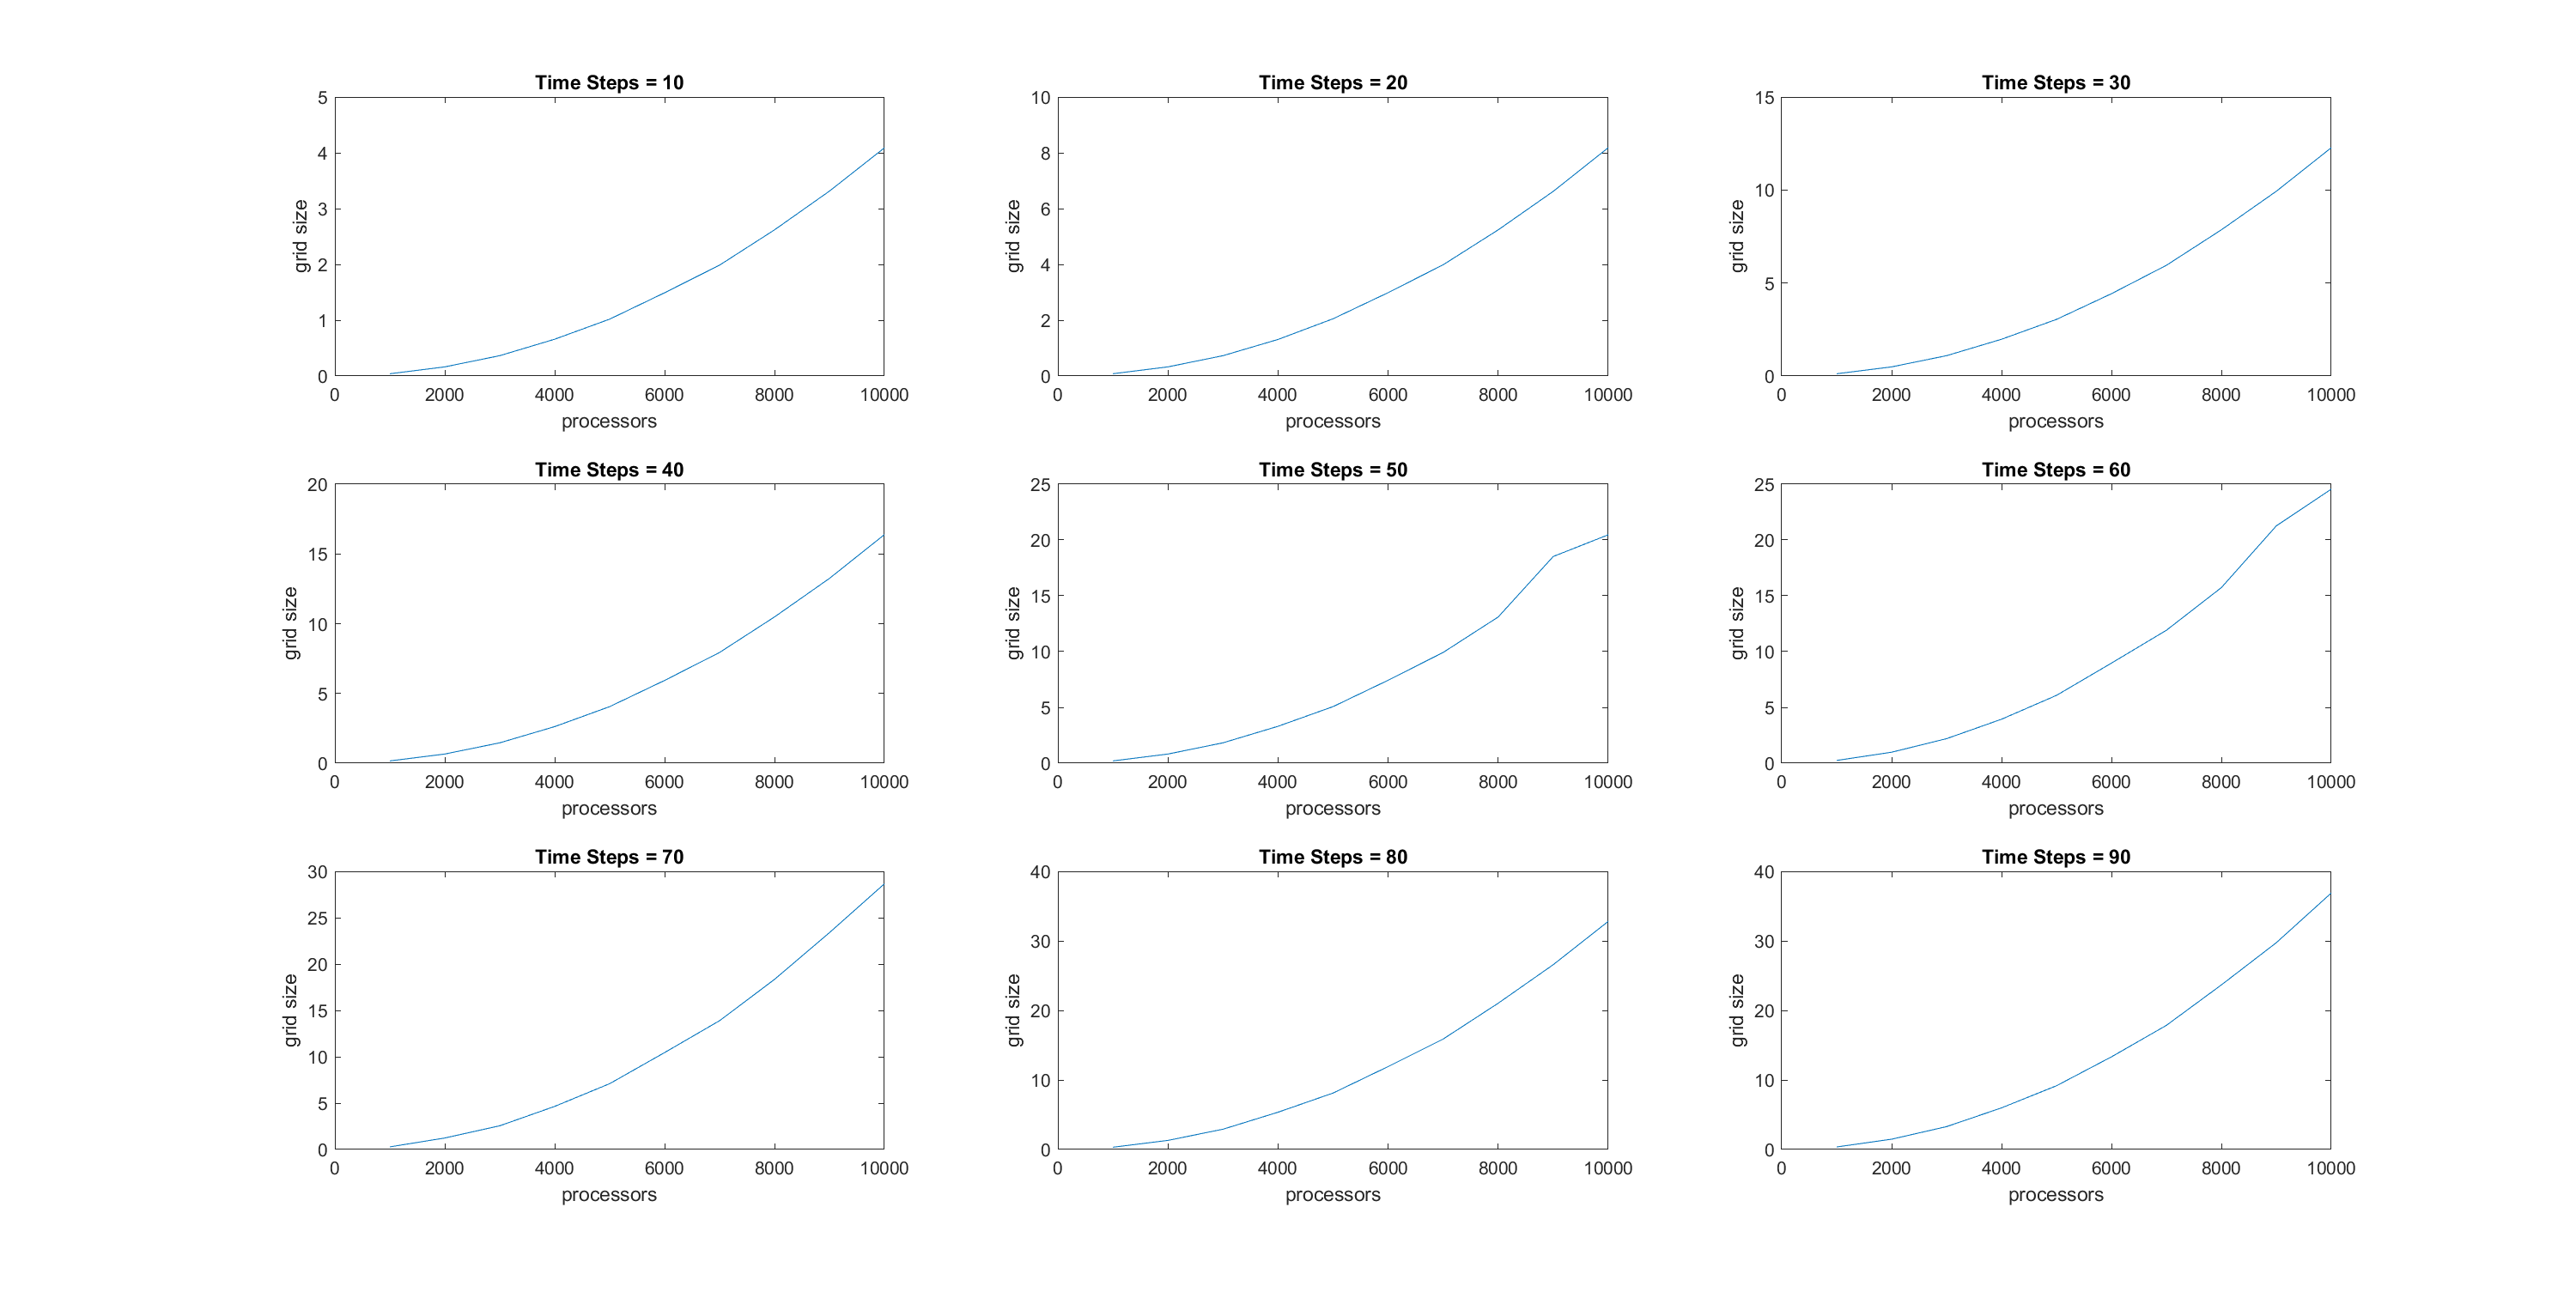
\includegraphics[width=7.5in]{serial_time.png}}
	\caption{Serial Runtimes for Given Time Steps}
\end{figure}

%---------------------------------------------------------------
% Section 2
%---------------------------------------------------------------
\section*{Parallel Runtime}
The figures within this section contain 3-dimensional meshes with the number of processors as the X axis, the grid size as the Y axis and time as the Z axis. In order to gain a perspective on the impact of the number of time steps on computation time, an adjusted version of each set of plots is included where the time axis is fixed above the maximum time value at 30.

As can be seen in the first set of graphs, the computation time when using MPI follows a mostly parabolic slope, but as the number of processors increases, the algorithm is not quite $O(n^2)$.
\begin{figure}[H]
	\centering
	\centerline{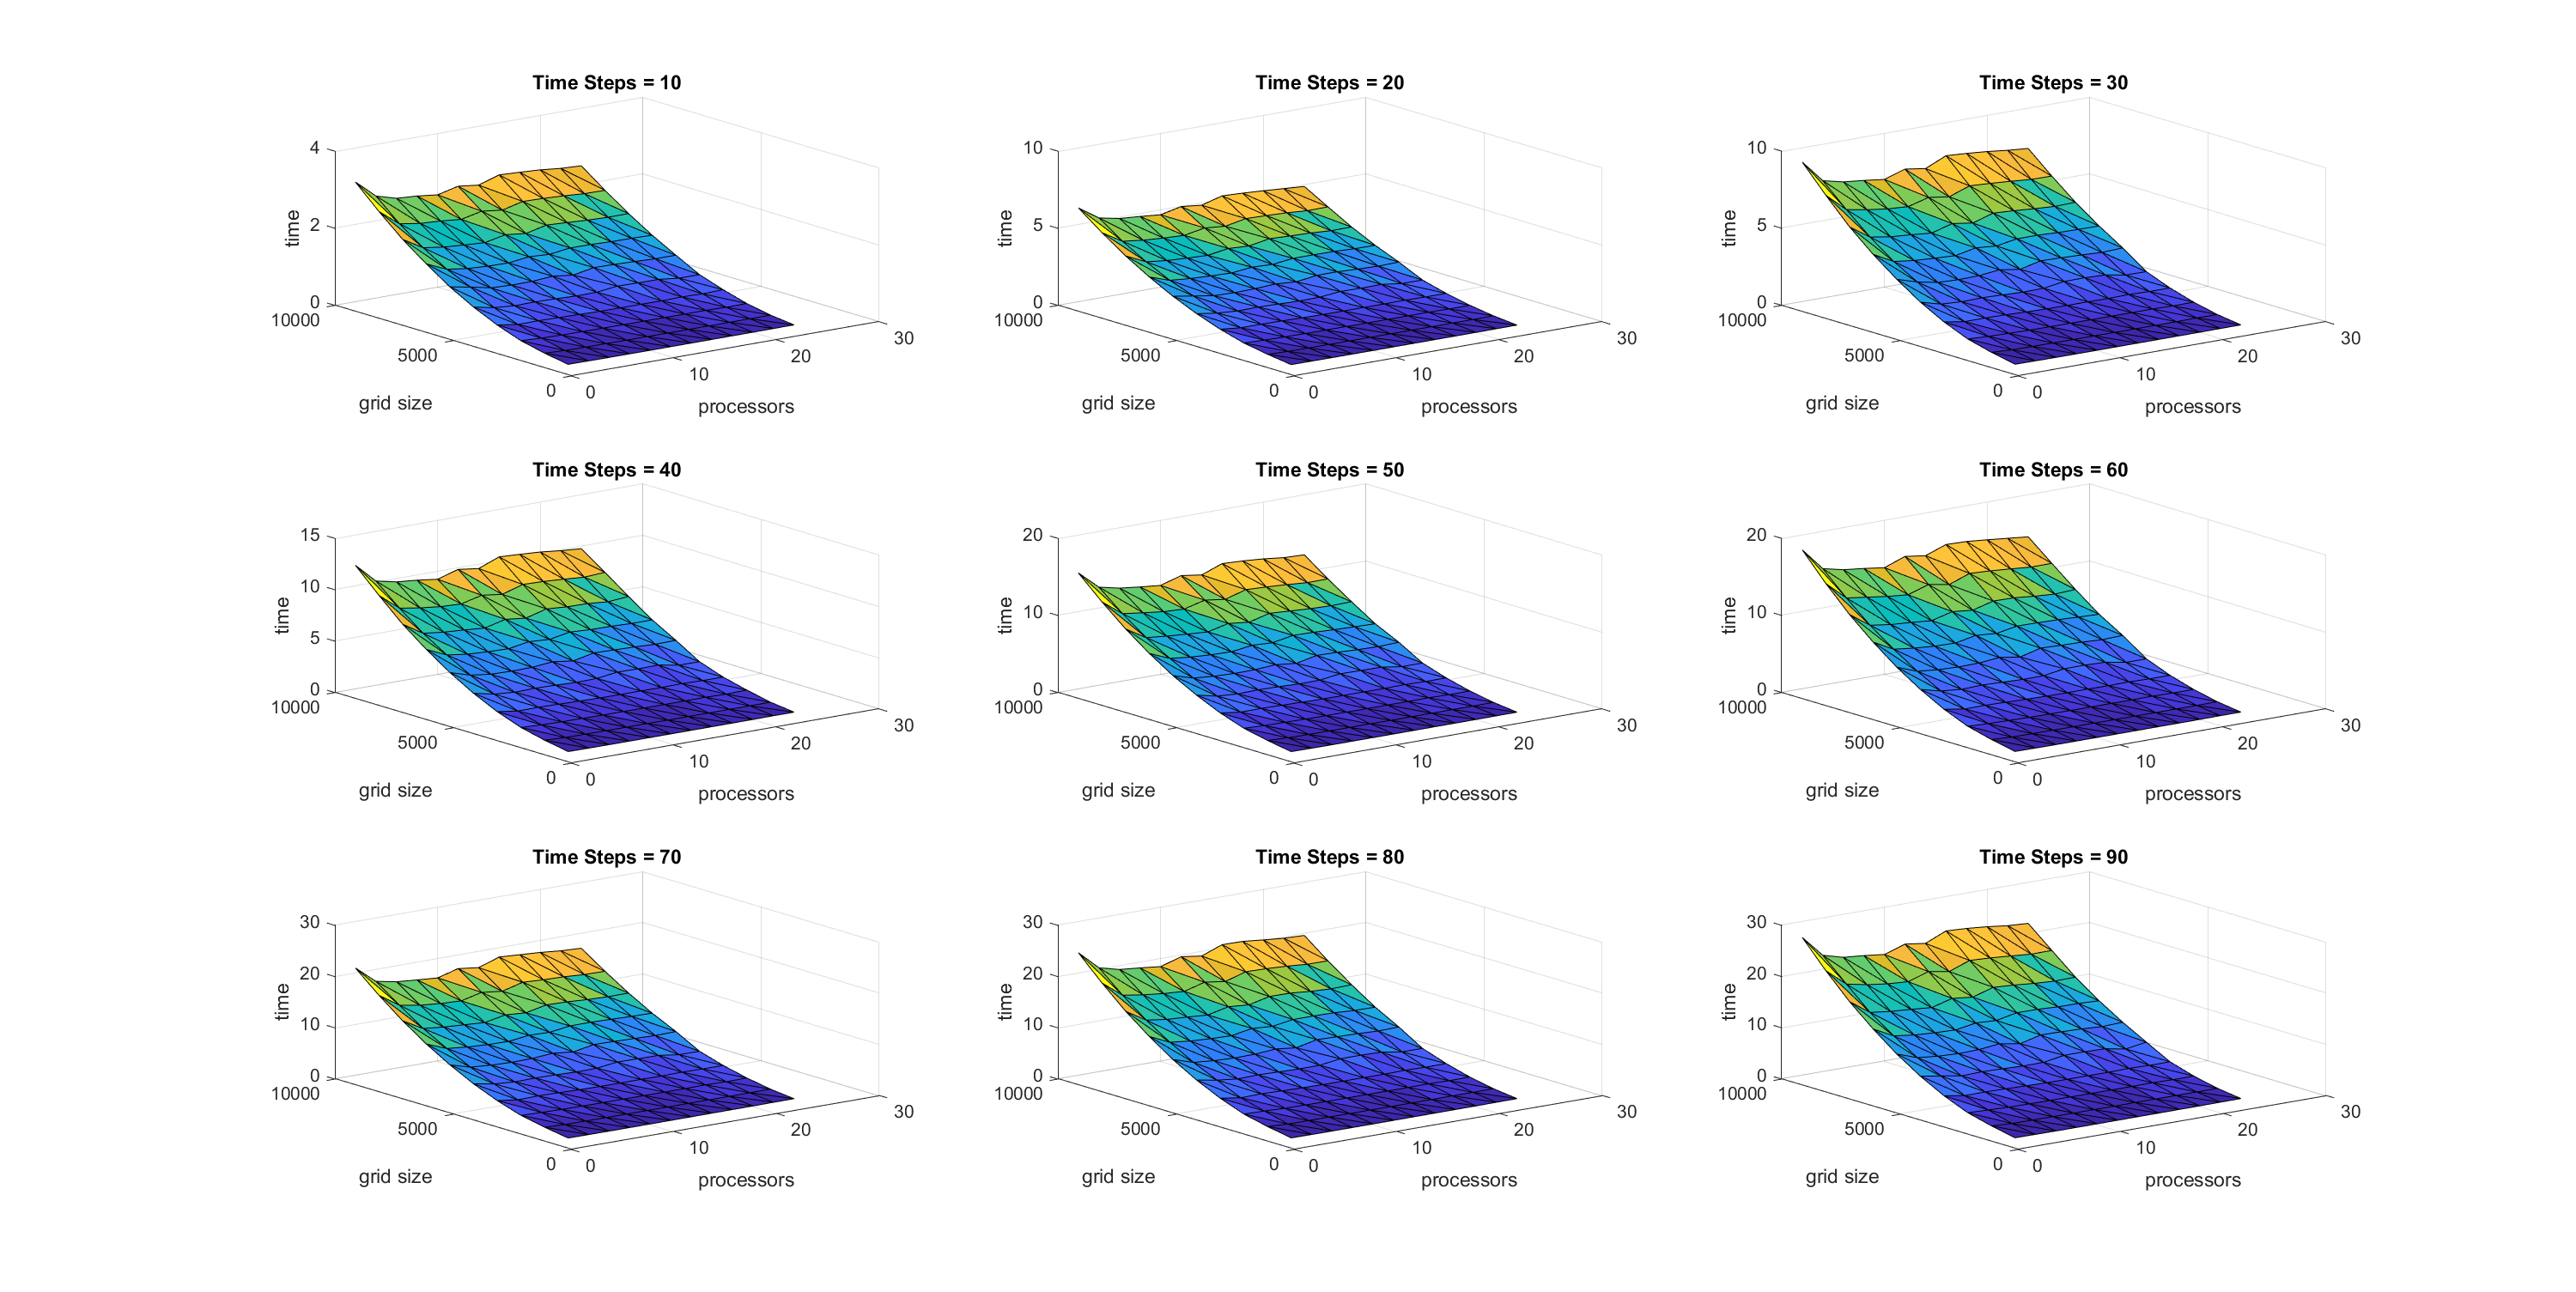
\includegraphics[width=7.5in]{parallel_time.png}}
	\caption{Parallel Runtimes for Given Time Steps}
\end{figure}

This figure contains the fixed z-axis height in order to provide a visual perspective on how detrimental the number of time steps is to the computation time.
\begin{figure}[H]
	\centering
	\centerline{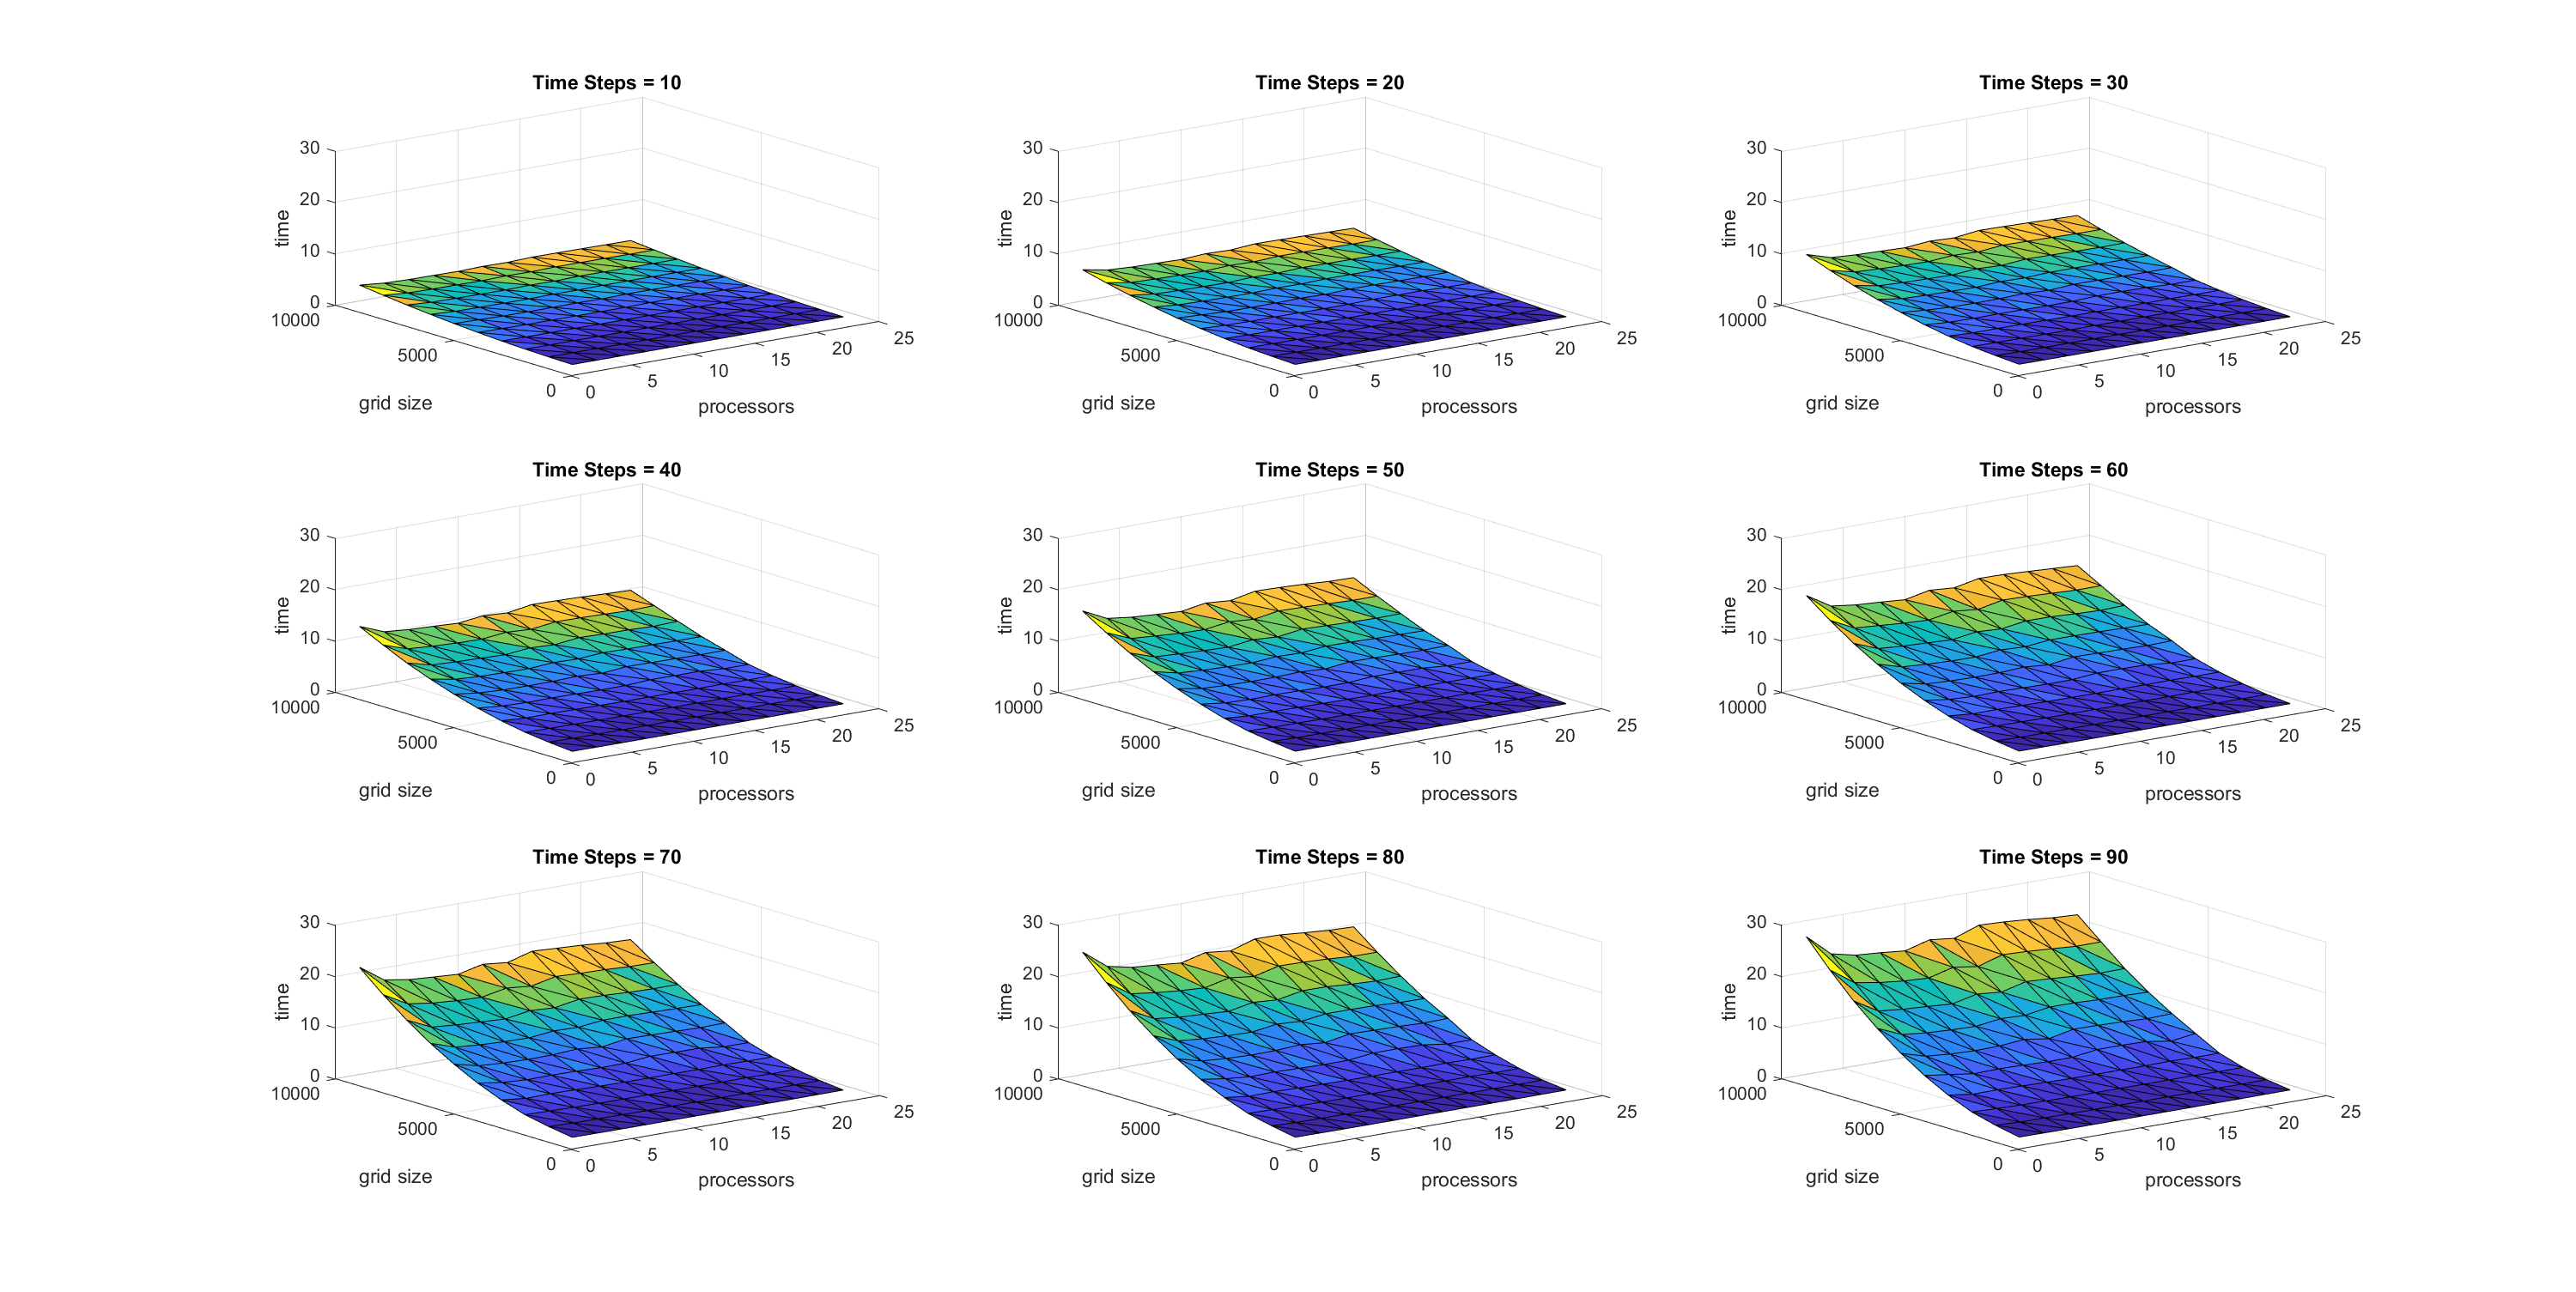
\includegraphics[width=7.5in]{parallel_time_scaled.png}}
	\caption{Parallel Runtimes for Given Time Steps (Scaled)}
\end{figure}

%---------------------------------------------------------------
% Section 3
%---------------------------------------------------------------
\section*{Parallel Communication Time}
For calculating the communication time, each processor created a timer before and after the MPI\_Sendrecv function calls, computed that time and printed it out into a file corresponding to it's rank. The data was then parsed using a python script in order to find the total communication time for each combination of:
\begin{itemize}
	\item Number of processors
	\item Grid size
	\item Time steps
\end{itemize}

For example, the communication time for rank 0 and rank 1 were added when $p=2$,$k=10$,$m=1000$ and so on.

Two pairs of graphs were created from this data. The first pair of graphs includes the absolute total communication time for each of the combinations, meaning that the time data point corresponding to $k=90$, $m=10,000$, $p=24$ contains the total communication time for all 24 processors. This data is presented below in the following two figures.
\begin{figure}[H]
	\centering
	\centerline{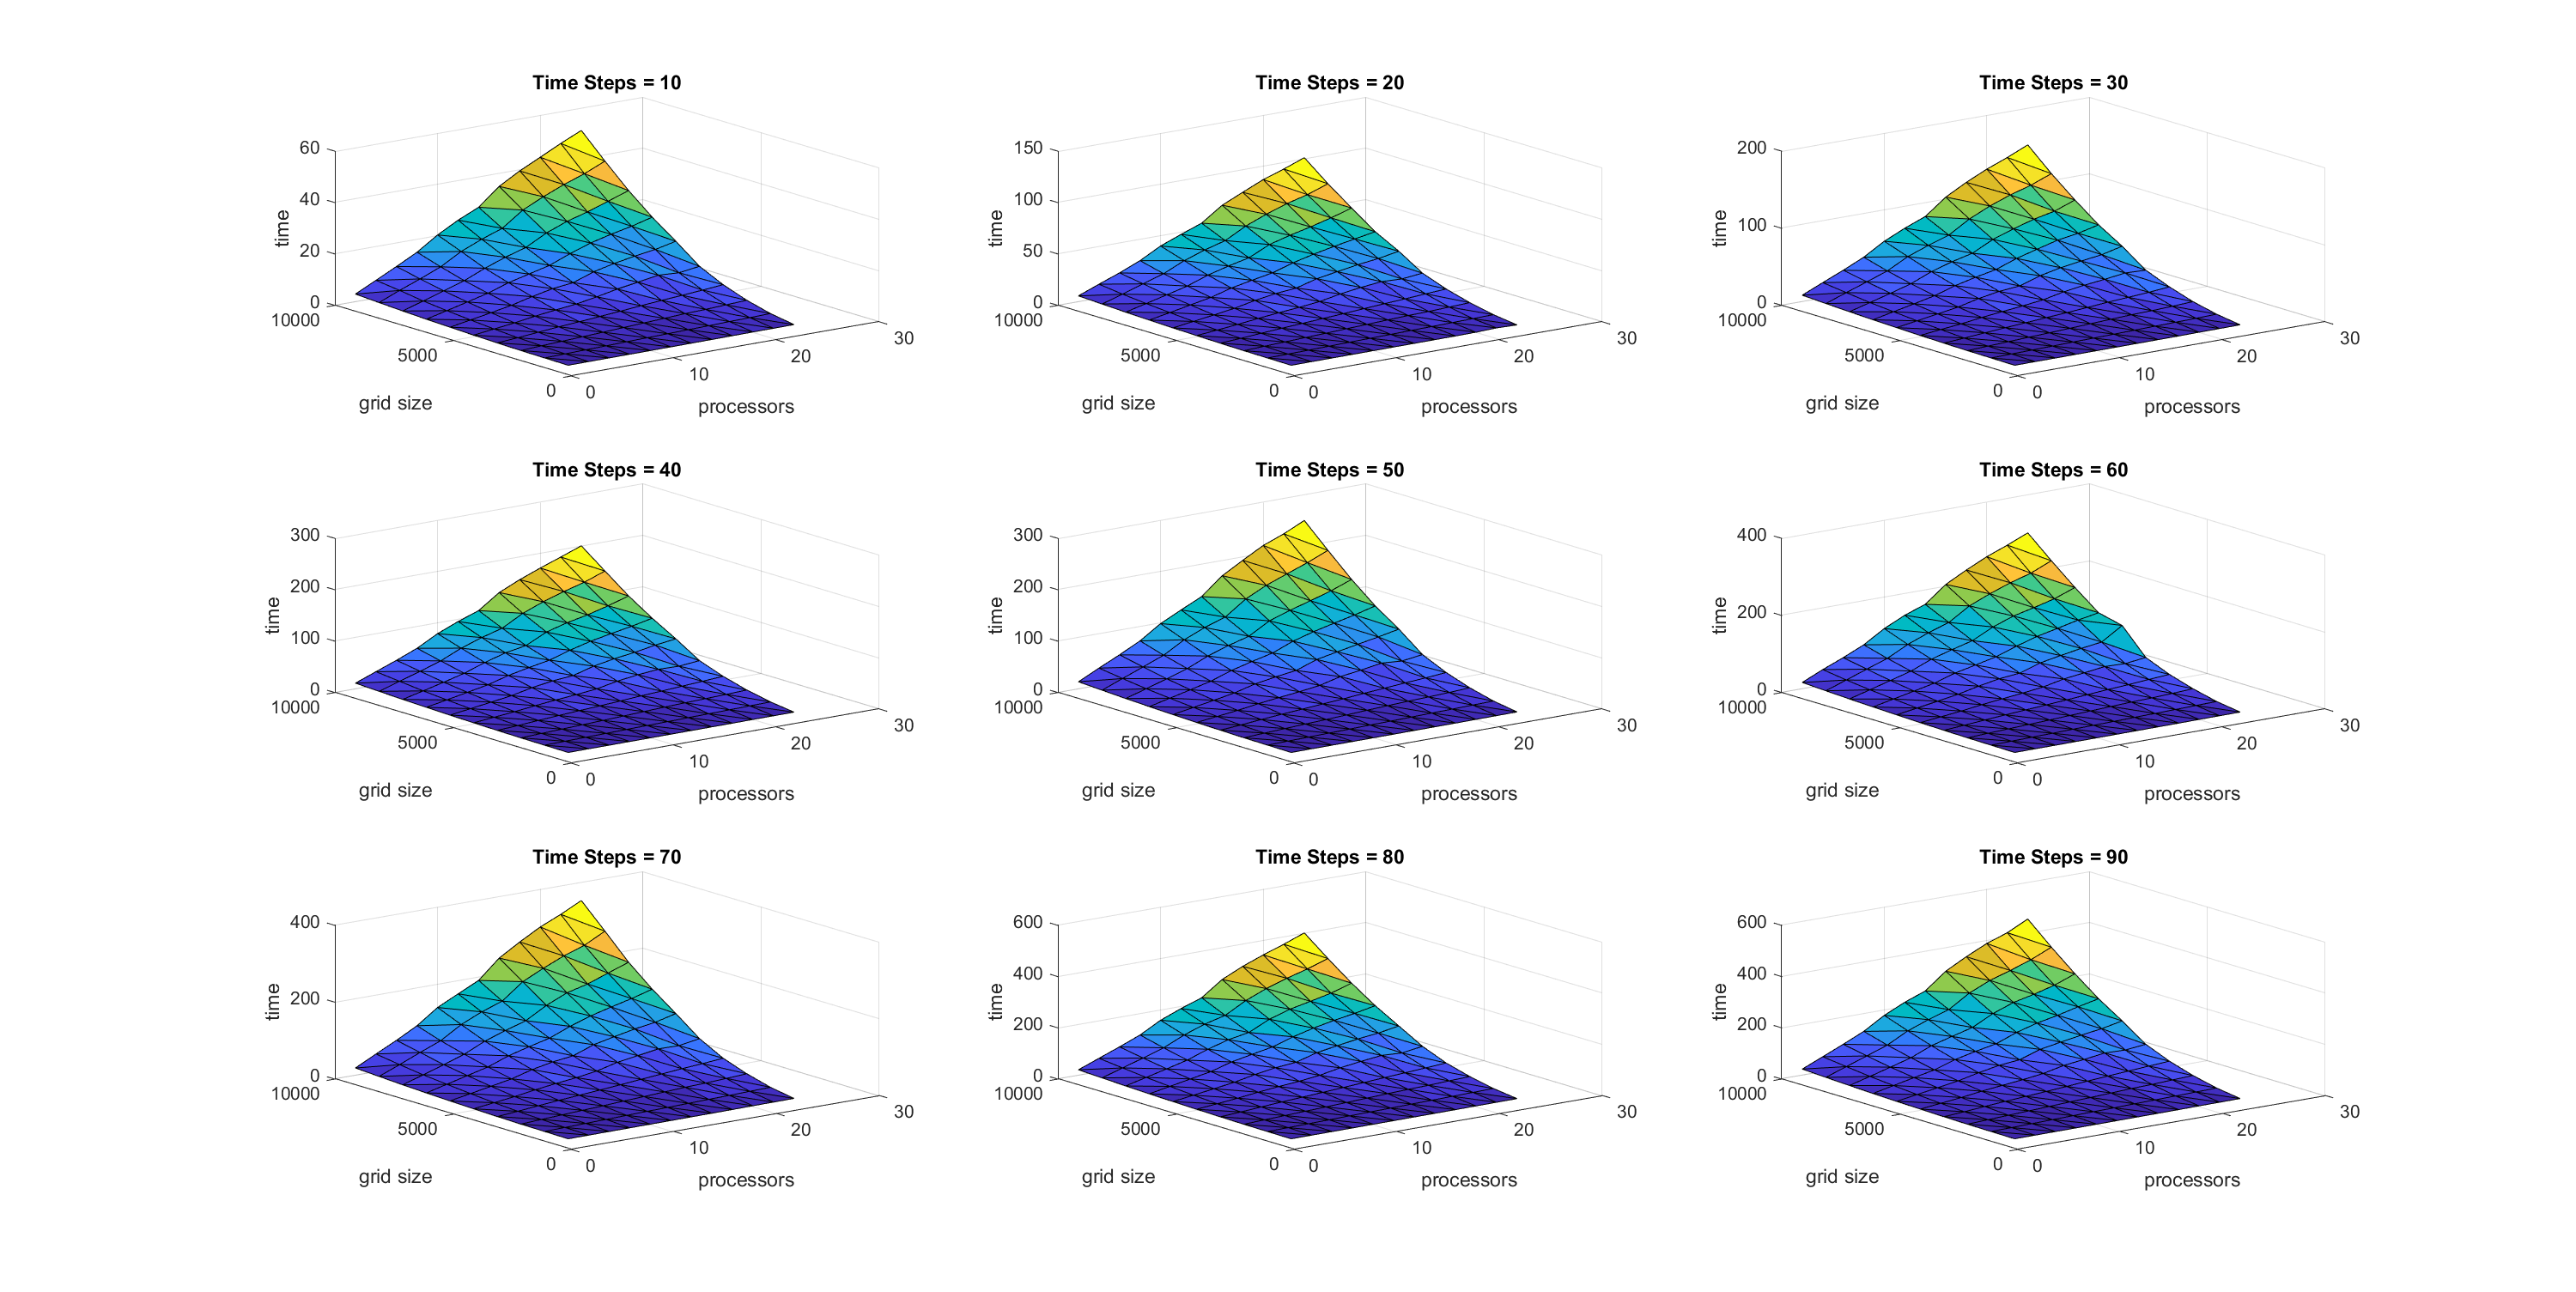
\includegraphics[width=7.5in]{comm_time.png}}
	\caption{Communication Time for Given Time Steps}
\end{figure}

The following set of graphs includes the same information as above, but with the time axis fixed at 500 seconds.

\begin{figure}[H]
	\centering
	\centerline{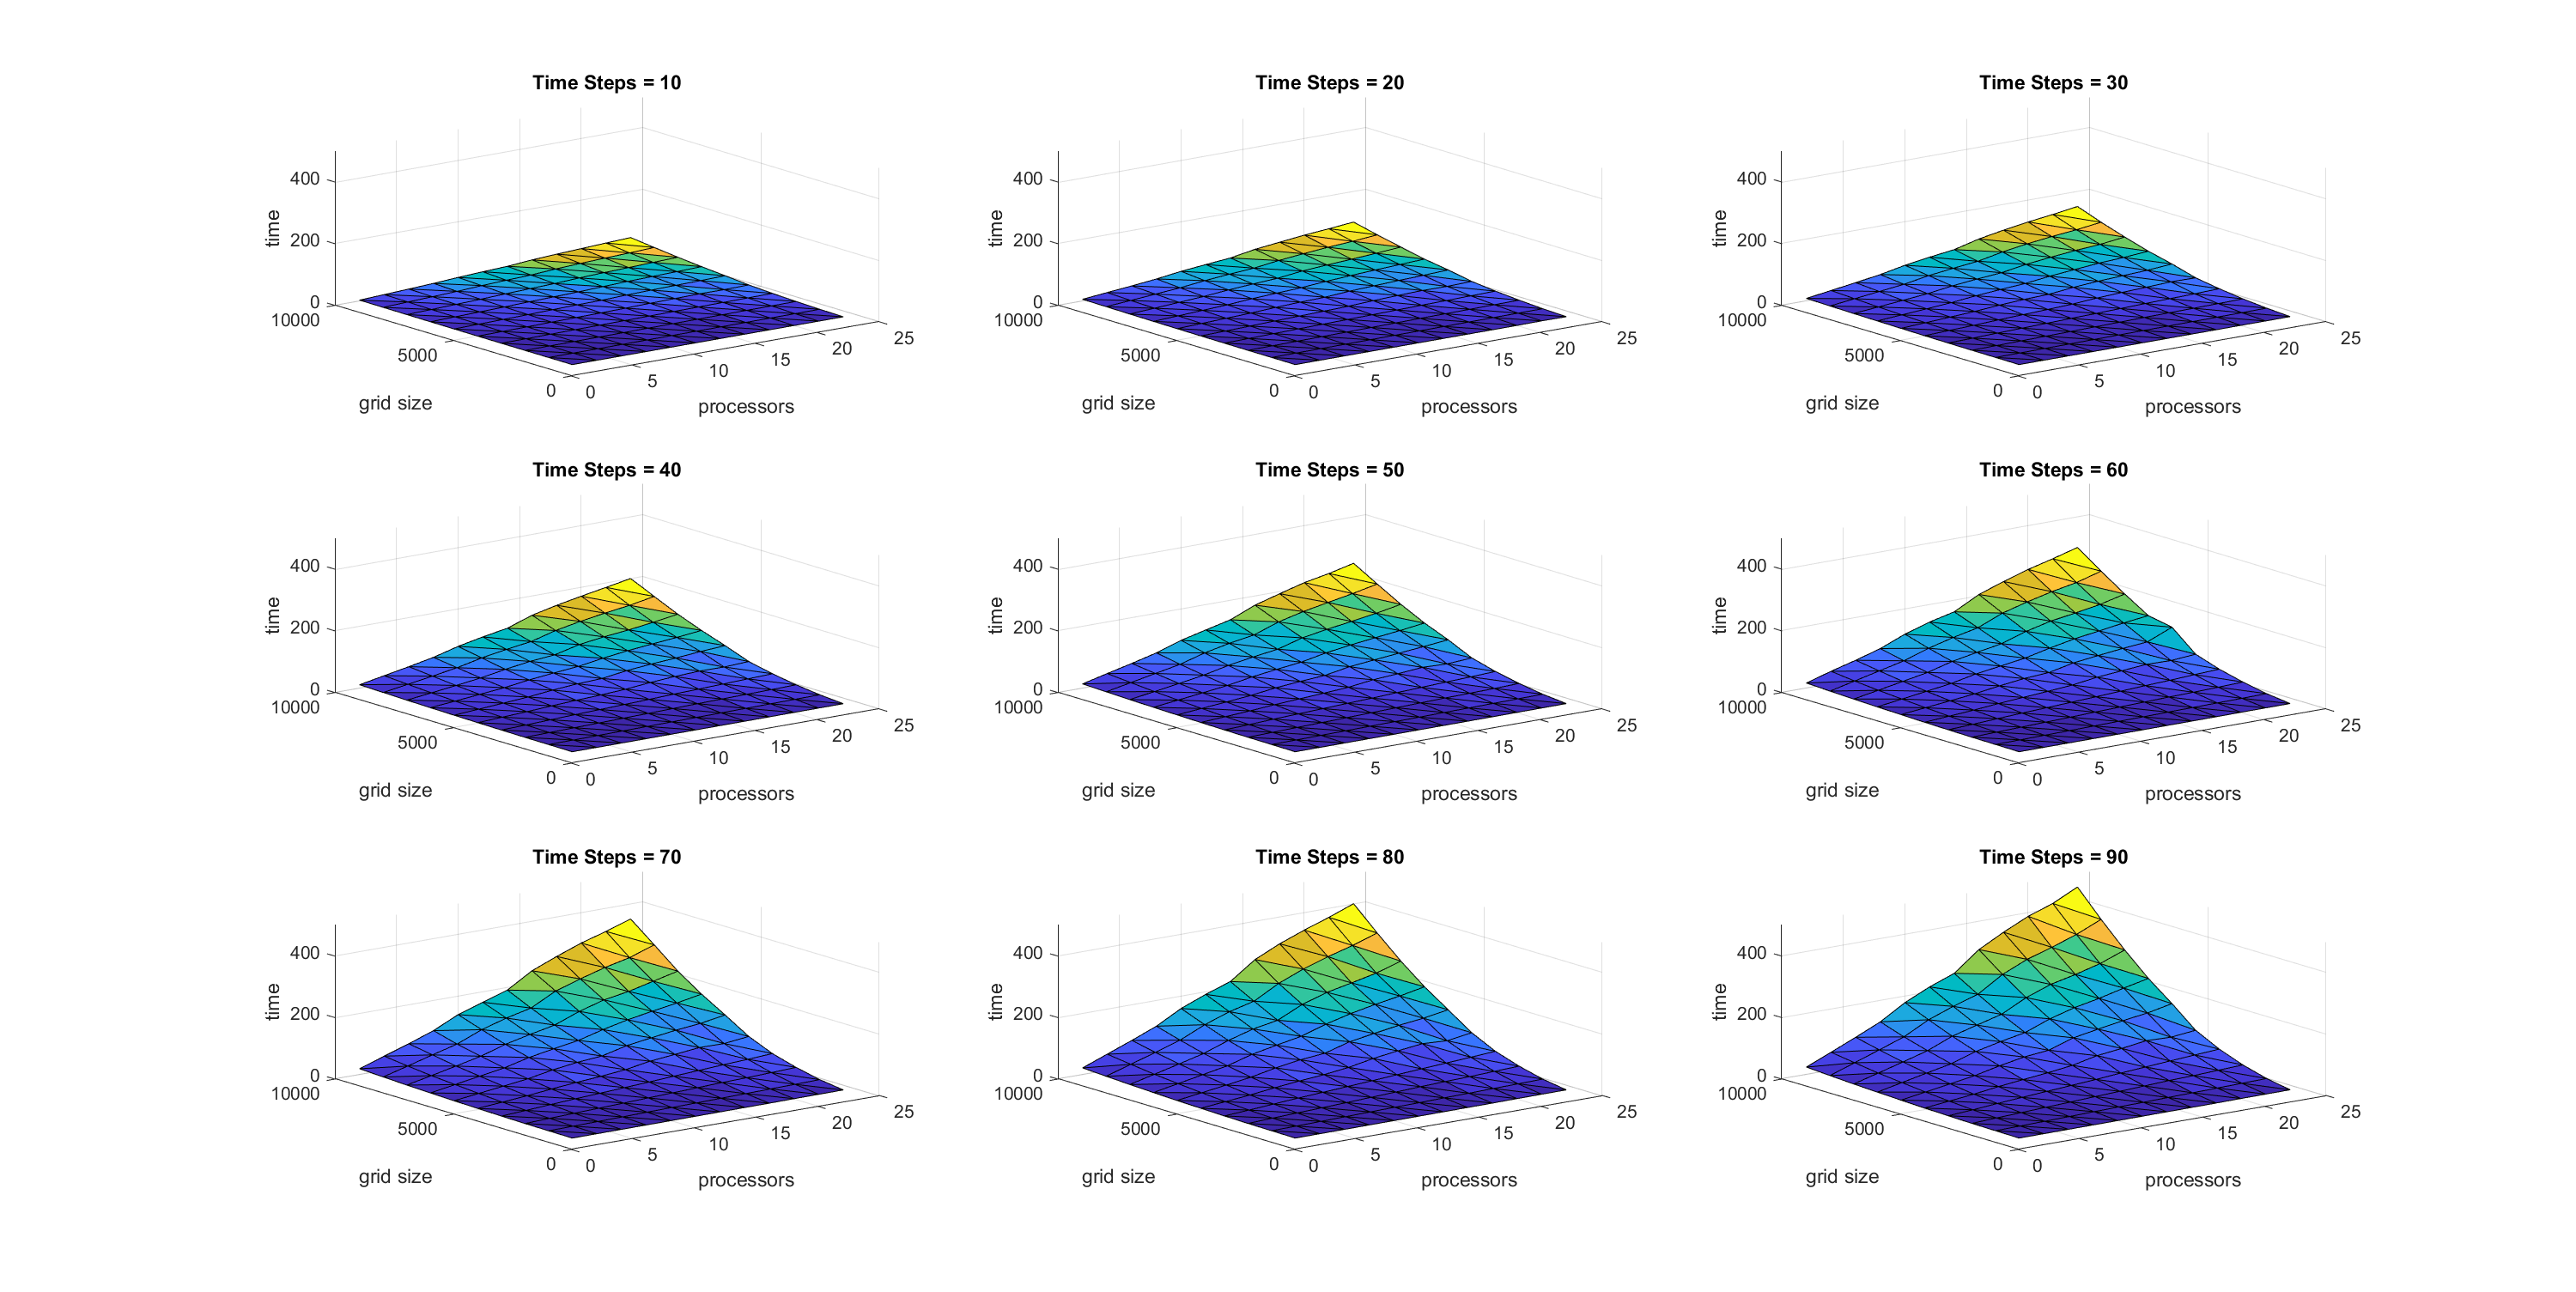
\includegraphics[width=7.5in]{comm_time_scaled.png}}
	\caption{Communication Time for Given Time Steps (Adjusted)}
\end{figure}

The second pair of graphs contain the average computation time per processor for each combination listed at the start of this section. It is interesting to note that, although the way the times were gathered is not perfect, at k=90, the communication times account for nearly 2/3 of the total run time.

\begin{figure}[H]
	\centering
	\centerline{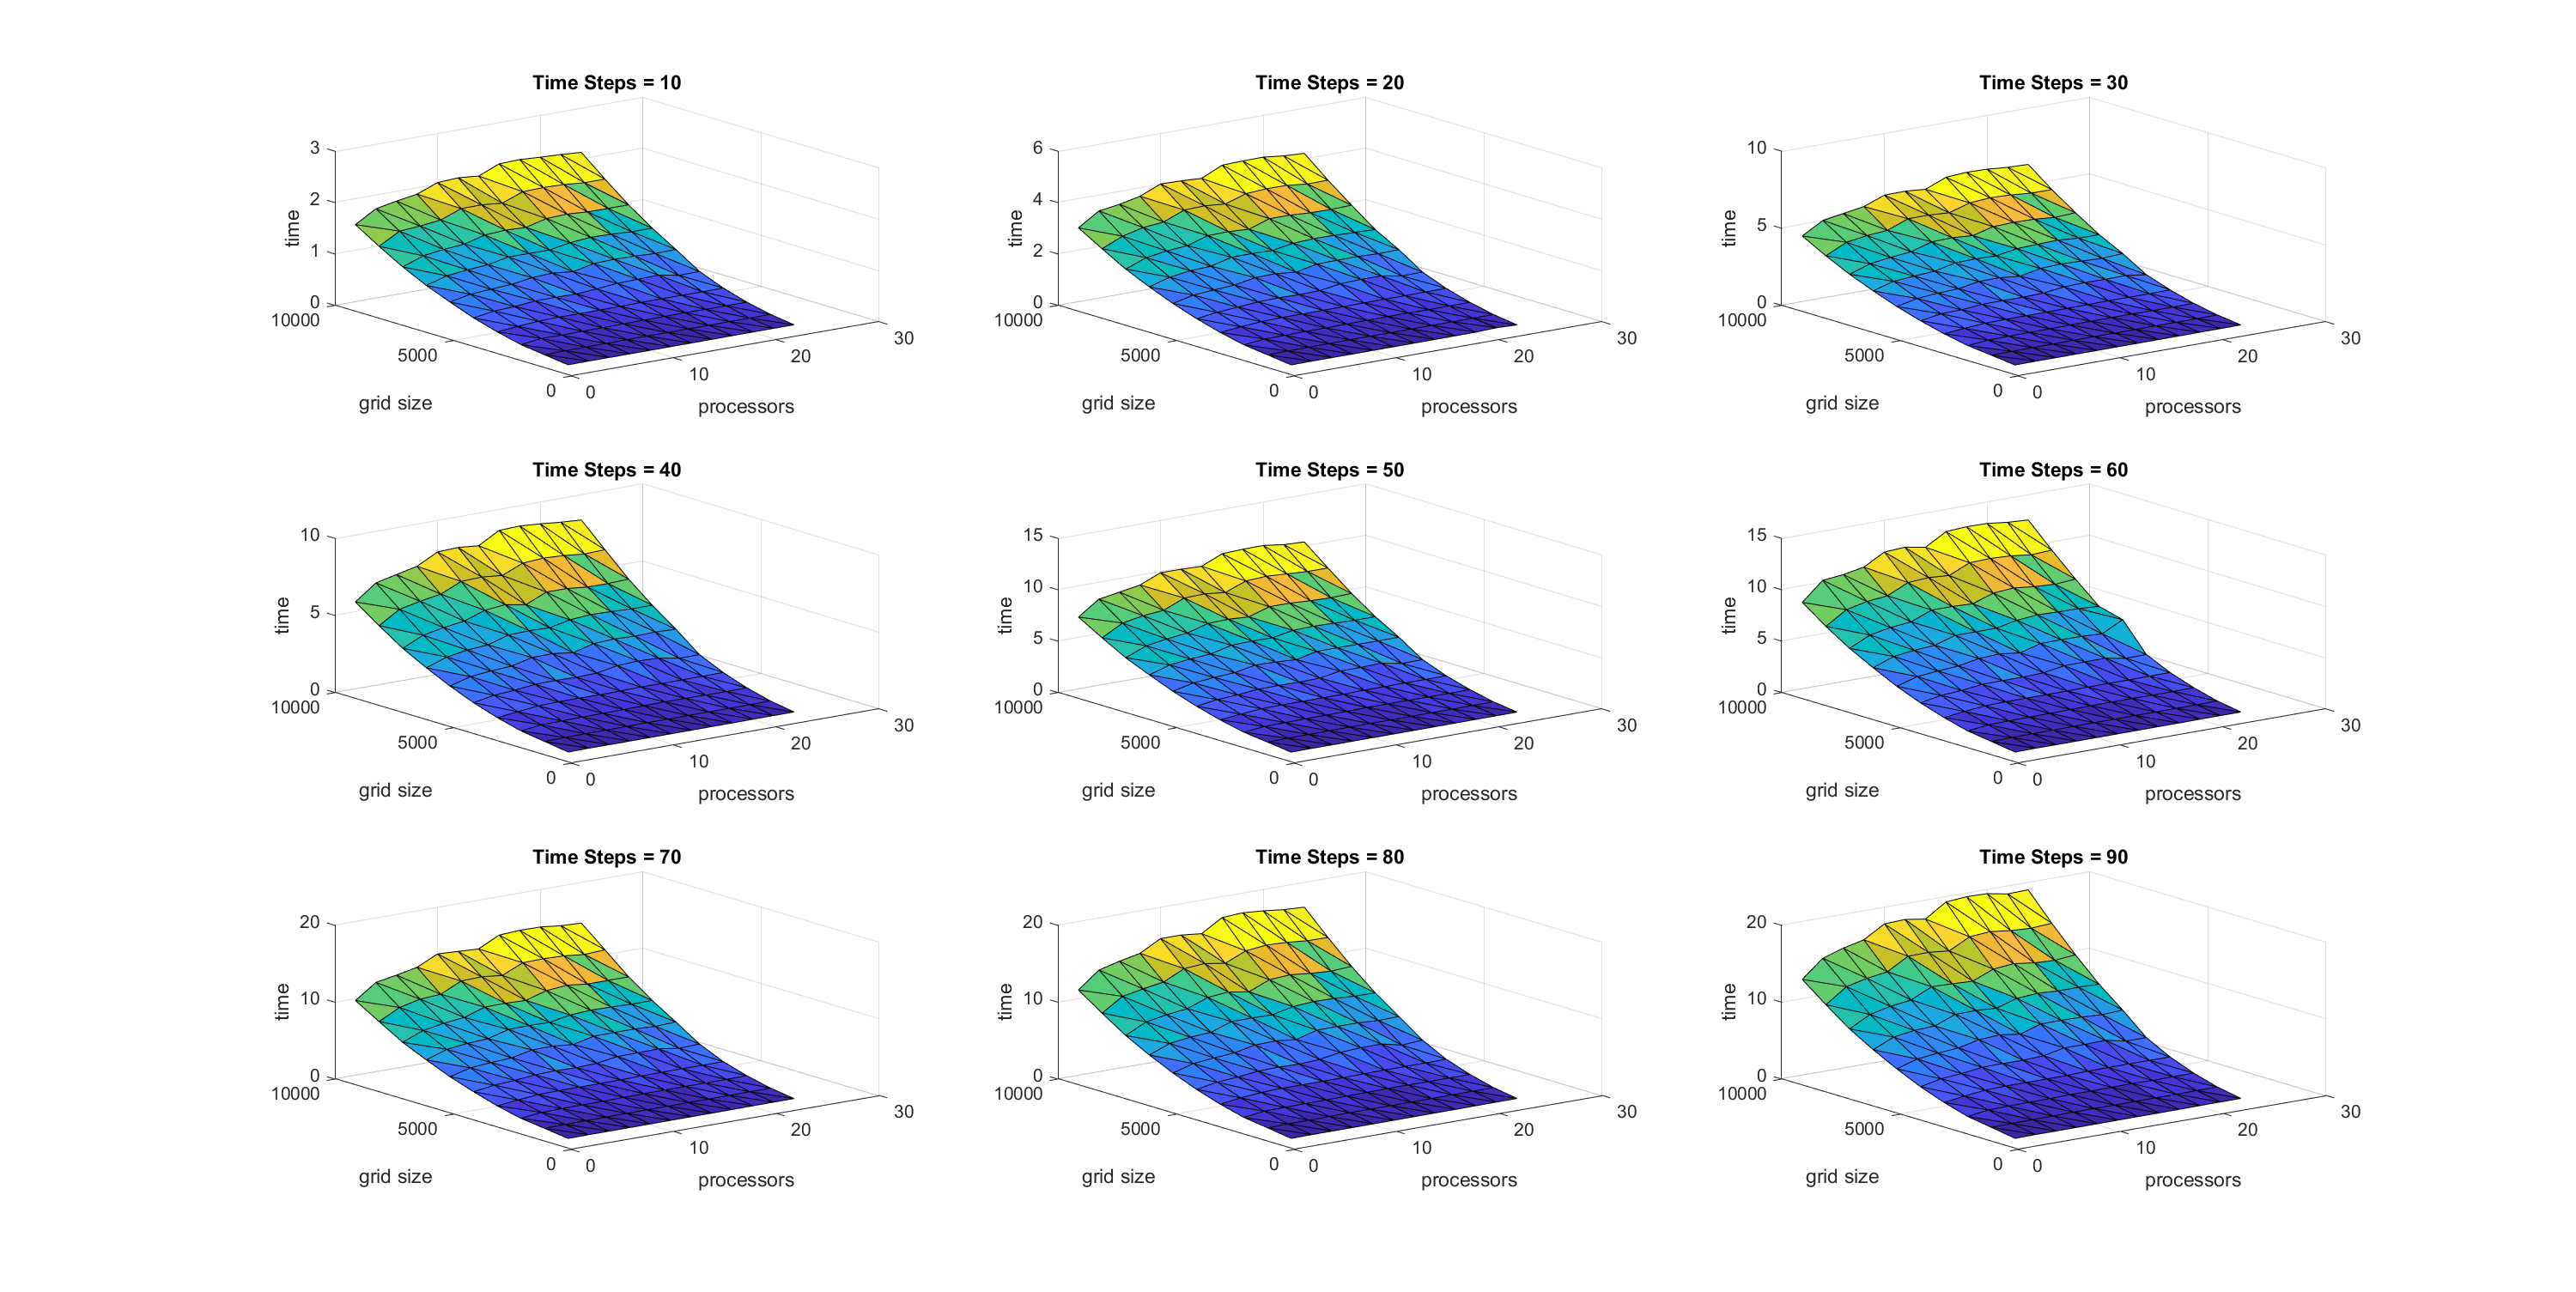
\includegraphics[width=7.5in]{comm_time_avg.png}}
	\caption{Average Communication Time for Given Time Steps}
\end{figure}

Again, in the following figure, the z axis is fixed in order to provide a perspective on the relative cost of increasing time steps.

\begin{figure}[H]
	\centering
	\centerline{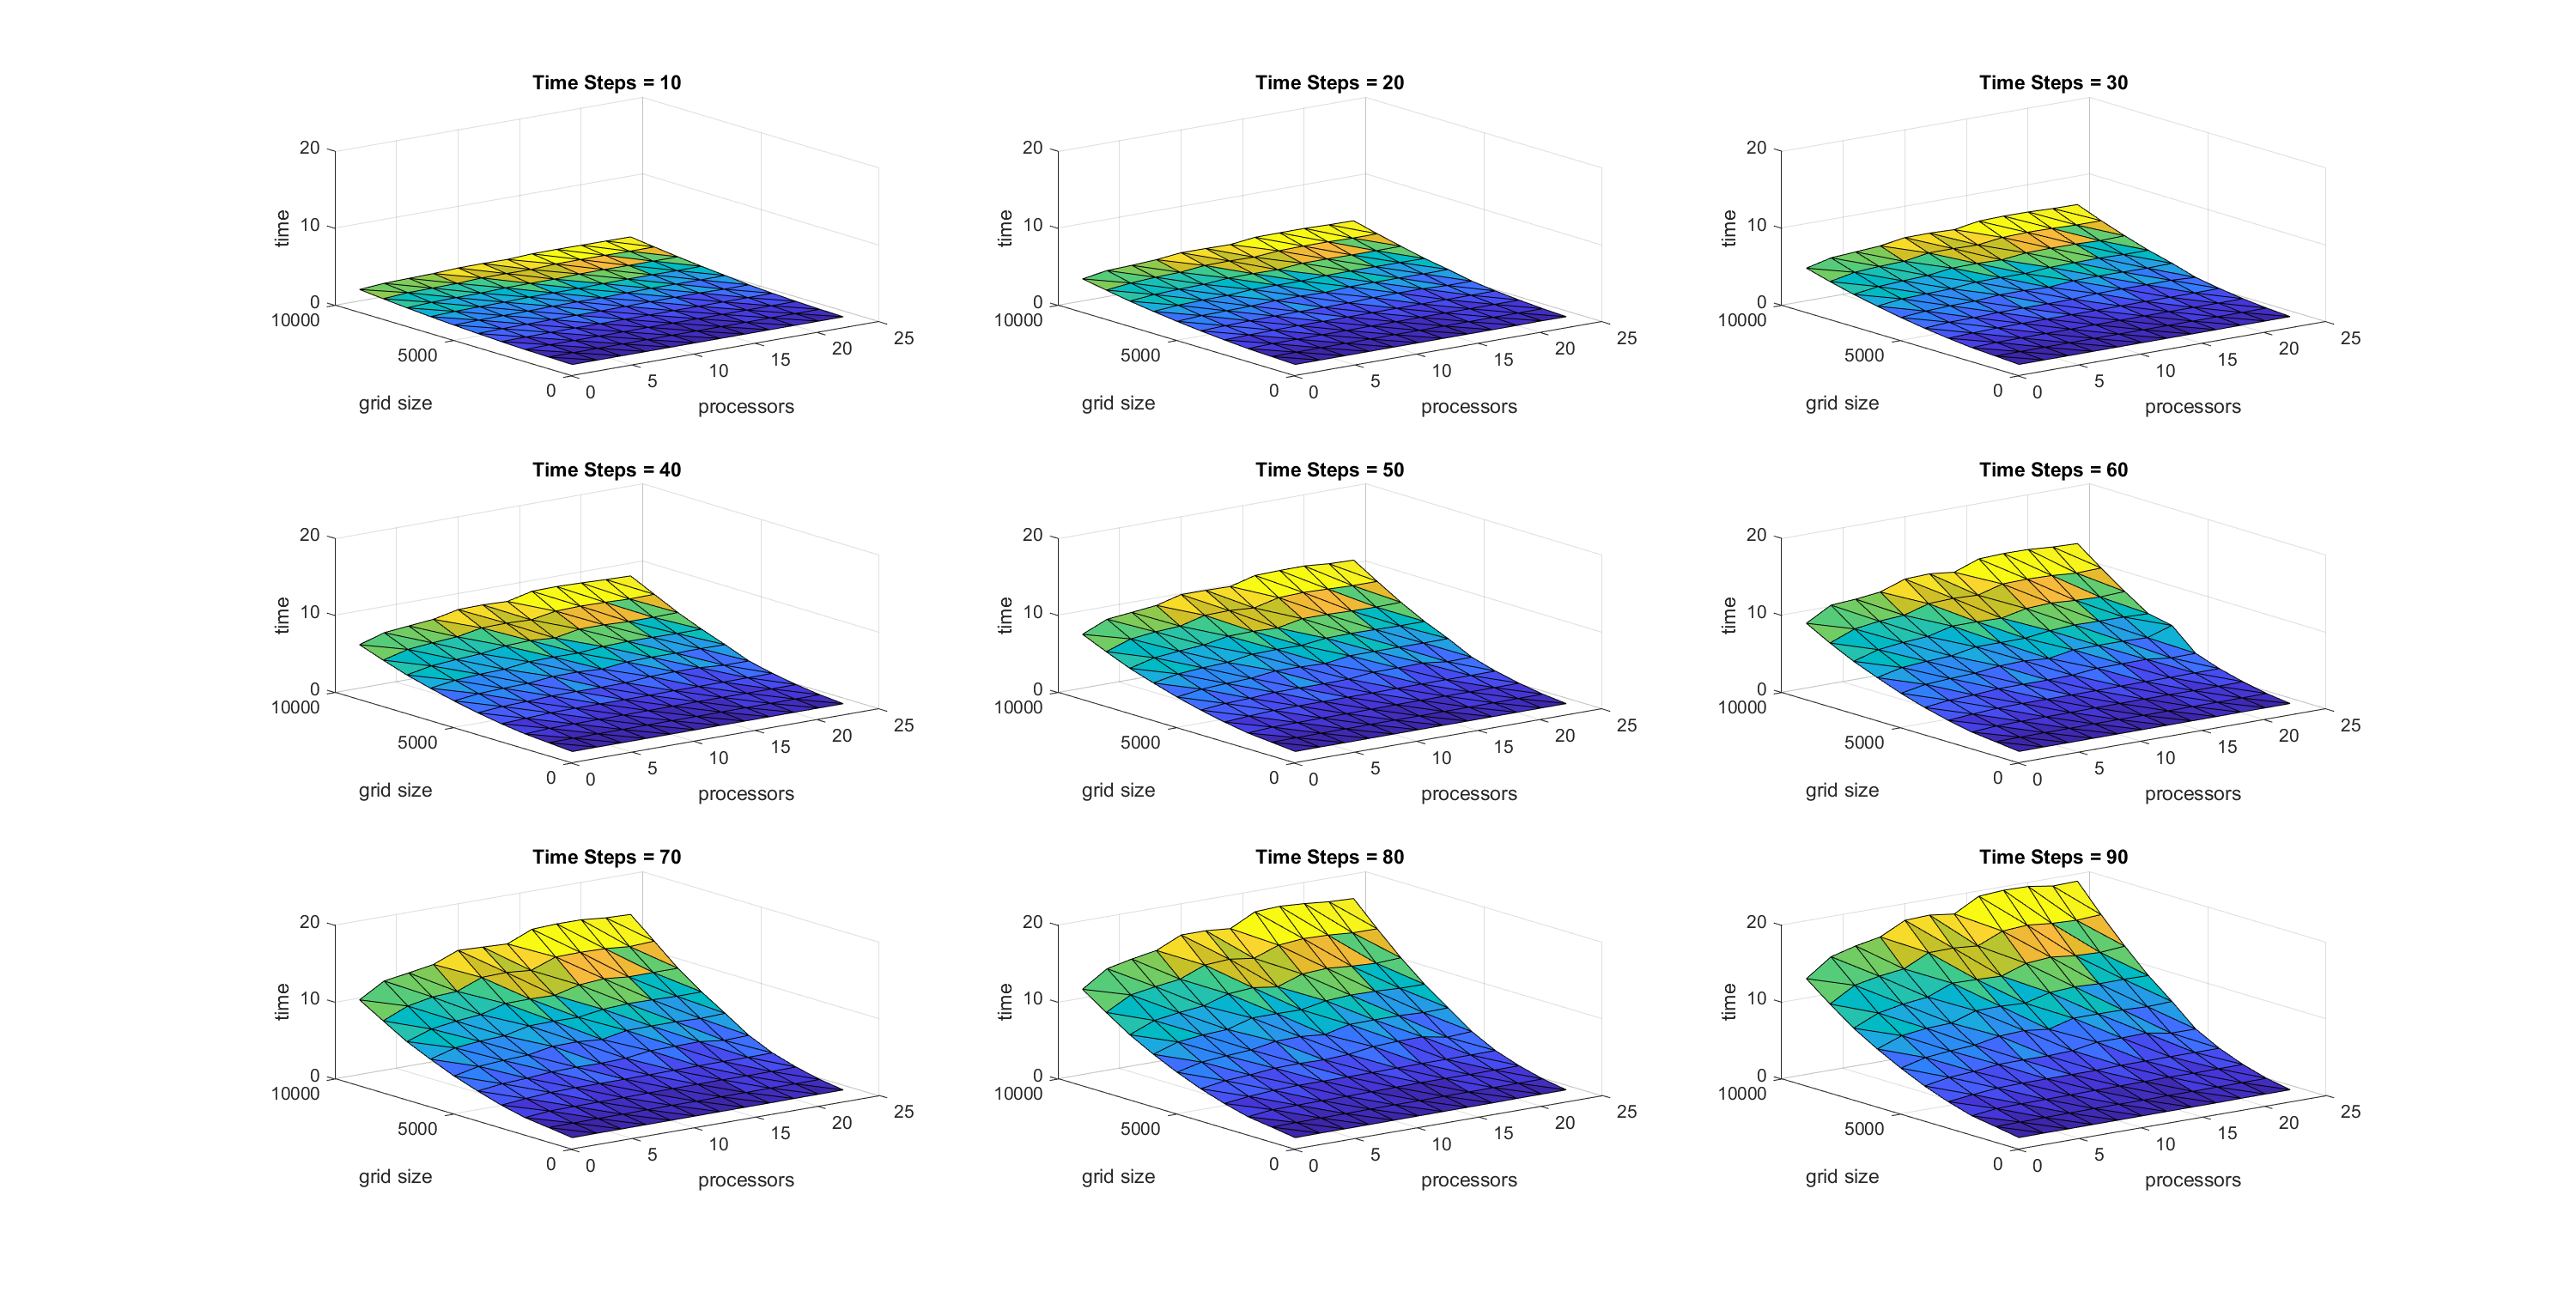
\includegraphics[width=7.5in]{comm_time_avg_scaled.png}}
	\caption{Average Communication Time for Given Time Steps (Adjusted)}
\end{figure}





%====================================================================
\newpage
\section*{MPI Code Appendix}
\lstinputlisting[language=C]{../main.c}

\newpage
\section*{Parse Code Appendix}
\lstinputlisting[language=Python]{../parse.py}

\newpage
\section*{Plotting Code Appendix}
\lstinputlisting[language=Matlab]{../plots.m}


\end{document}